% Remember to input this to the presentative tex file before compiling.
\chapter{Conclusion}
\begin{itemize}
    \item The aim of the project involves multi-sensor data analysis and designing a set-up to characterise devices for the identification of gases. 
    \item The data collected with 3 sensor arrays was analysed using machine learning techniques.
    \item The main method for analysis relied on the dimensional reduction method to visualise data and ML methods for the classification of the data.
    \item The comparison of the classification results using various methods like Decision tree, Random forest and NN was performed and the same is listed in Figure 6.1.
    \item Almost all training data could be predicted with an accuracy of above 90\%. However, the decision tree model gave the fastest result compared to other models.
    \item A new setup that can record the response data for six sensors simultaneously, with individual heater control for each sensor, has been designed and developed.
\end{itemize}

\begin{figure}
    \centering
    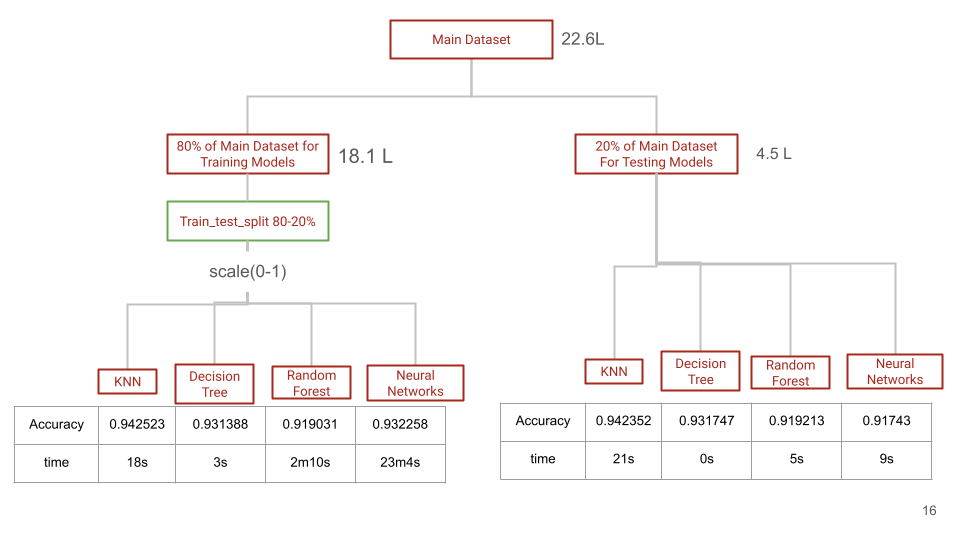
\includegraphics[width=1\linewidth]{Thesis Prashant//Images//Results/Classifier Results.png}
    \caption{Model Comparison on training and unknown data set}
    \label{fig:enter-label}
\end{figure}

%The results for different classification methods give accuracy during training period KNN $94.25\%$, Decision Tree  $93.13\%$, Random Forest $91.90\%$, and Neural Networks $93.22\%$  in time 18s, 3s, 2min, and 23min respectively. And while using the exported model on a completely unknown data set  KNN $94.23\%$, Decision Tree  $93.17\%$, Random Forest $91.92\%$, and Neural Networks $91.74\%$ in time 21s, ~0s, 5s, and 9s respectively.








